\lhead{4. Tries}

\begin{enumerate}[label=\textbf{\Alph*.}]

\item \textbf{Define Trie Data Structure and its Importance in String Processing.}

A Trie, also known as a Prefix Tree, is a tree-based data structure used to store
and retrieve strings efficiently.

In a Trie:
\begin{itemize}
\item Each node represents a character.
\item Words sharing common prefixes use the same path.
\item Special markers indicate the end of words.
\end{itemize}

\textbf{Importance}
\begin{itemize}
\item Fast searching of words.
\item Efficient storage of strings.
\item Useful for prefix matching.
\item Widely used in dictionaries and search systems.
\end{itemize}

\item \textbf{List any two applications of Trie.}

\begin{enumerate}[label=\textbf{\arabic*.}]
\item \textbf{Autocomplete Systems}\\
Used in search engines and mobile keyboards to suggest words while typing.

\item \textbf{Spell Checking}\\
Used to verify whether a word exists in a dictionary.
\end{enumerate}

\item \textbf{Explain insertion and searching operations in a Trie with suitable examples.}



\item \textbf{Construct a Trie for the following set of words:
\begin{center}CAT, CAR, CARE, DOG\end{center}}

\begin{enumerate}[label=\arabic*.]                                                                                                                                                              \item Initial Trie:
\begin{center}
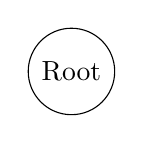
\begin{tikzpicture}[
  level 1/.style={sibling distance=4cm},
  level 2/.style={sibling distance=2cm},
  level 3/.style={sibling distance=1.5cm},
  edge from parent/.style={draw,-},
  every node/.style={circle, draw, minimum size=8mm}
]
\node {Root};
\end{tikzpicture}
\end{center}

\item Inserting "CAT":

\begin{center}
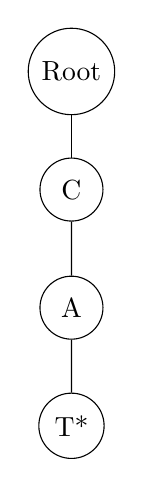
\begin{tikzpicture}[
  level 1/.style={sibling distance=4cm},
  level 2/.style={sibling distance=2cm},
  level 3/.style={sibling distance=1.5cm},
  edge from parent/.style={draw,-},
  every node/.style={circle, draw, minimum size=8mm}
]
\node {Root}
  child { node {C}
    child { node {A}
      child { node {T*}}
    }
  };
\end{tikzpicture}
\end{center}

\textit{\textbf{NOTE:} The {"*"} denotes the end-of-word marker.}

\item Inserting "CAR":

\begin{center}
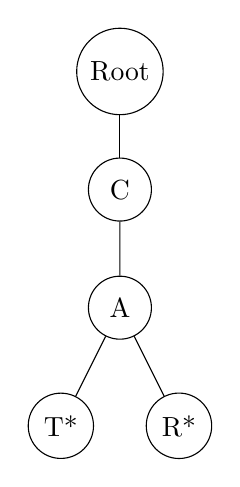
\begin{tikzpicture}[
  level 1/.style={sibling distance=4cm},
  level 2/.style={sibling distance=2cm},
  level 3/.style={sibling distance=1.5cm},
  edge from parent/.style={draw,-},
  every node/.style={circle, draw, minimum size=8mm}
]
\node {Root}
  child { node {C}
    child { node {A}
      child { node {T*} }
      child { node {R*} }
    }
  };
\end{tikzpicture}
\end{center}

\item Inserting "CARE":

\begin{center}
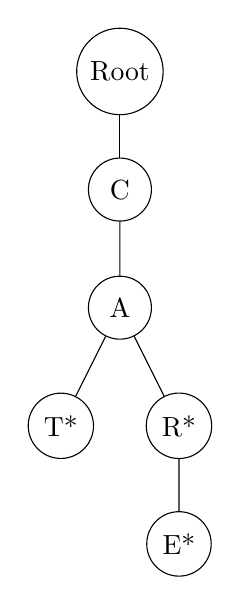
\begin{tikzpicture}[
  level 1/.style={sibling distance=4cm},
  level 2/.style={sibling distance=2cm},
  level 3/.style={sibling distance=1.5cm},
  edge from parent/.style={draw,-},
  every node/.style={circle, draw, minimum size=8mm}
]
\node {Root}
  child { node {C}
    child { node {A}
      child { node {T*} }
      child { node {R*}
        child { node {E*} }
      }
    }
  };
\end{tikzpicture}
\end{center}

\item Inserting "DOG":

\begin{center}
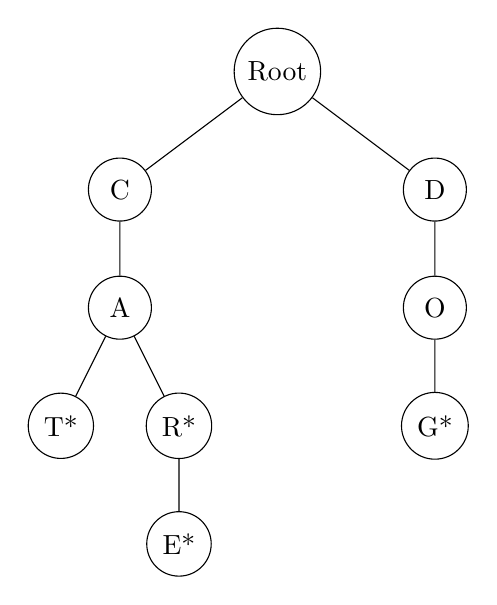
\begin{tikzpicture}[
  level 1/.style={sibling distance=4cm},
  level 2/.style={sibling distance=2cm},
  level 3/.style={sibling distance=1.5cm},
  edge from parent/.style={draw,-},
  every node/.style={circle, draw, minimum size=8mm}
]

\node {Root}
  child { node {C}
    child { node {A}
      child { node {T*} }
      child { node {R*}
        child { node {E*} }
      }
    }
  }
  child { node {D}
      child { node {O}
      child { node {G*} }
    }
  };

\end{tikzpicture}
\end{center}
\end{enumerate}
\end{enumerate}

\begin{center}
\vspace{1cm}
$\ast \ast \ast$
\end{center}
